\documentclass[]{article}
\usepackage{lmodern}
\usepackage{amssymb,amsmath}
\usepackage{ifxetex,ifluatex}
\usepackage{fixltx2e} % provides \textsubscript
\ifnum 0\ifxetex 1\fi\ifluatex 1\fi=0 % if pdftex
  \usepackage[T1]{fontenc}
  \usepackage[utf8]{inputenc}
\else % if luatex or xelatex
  \ifxetex
    \usepackage{mathspec}
  \else
    \usepackage{fontspec}
  \fi
  \defaultfontfeatures{Ligatures=TeX,Scale=MatchLowercase}
\fi
% use upquote if available, for straight quotes in verbatim environments
\IfFileExists{upquote.sty}{\usepackage{upquote}}{}
% use microtype if available
\IfFileExists{microtype.sty}{%
\usepackage{microtype}
\UseMicrotypeSet[protrusion]{basicmath} % disable protrusion for tt fonts
}{}
\usepackage[margin=1in]{geometry}
\usepackage{hyperref}
\hypersetup{unicode=true,
            pdftitle={3rd Assignment. Frank Wolfe algorithm},
            pdfauthor={Arnau Mercader Luque},
            pdfborder={0 0 0},
            breaklinks=true}
\urlstyle{same}  % don't use monospace font for urls
\usepackage{graphicx,grffile}
\makeatletter
\def\maxwidth{\ifdim\Gin@nat@width>\linewidth\linewidth\else\Gin@nat@width\fi}
\def\maxheight{\ifdim\Gin@nat@height>\textheight\textheight\else\Gin@nat@height\fi}
\makeatother
% Scale images if necessary, so that they will not overflow the page
% margins by default, and it is still possible to overwrite the defaults
% using explicit options in \includegraphics[width, height, ...]{}
\setkeys{Gin}{width=\maxwidth,height=\maxheight,keepaspectratio}
\IfFileExists{parskip.sty}{%
\usepackage{parskip}
}{% else
\setlength{\parindent}{0pt}
\setlength{\parskip}{6pt plus 2pt minus 1pt}
}
\setlength{\emergencystretch}{3em}  % prevent overfull lines
\providecommand{\tightlist}{%
  \setlength{\itemsep}{0pt}\setlength{\parskip}{0pt}}
\setcounter{secnumdepth}{0}
% Redefines (sub)paragraphs to behave more like sections
\ifx\paragraph\undefined\else
\let\oldparagraph\paragraph
\renewcommand{\paragraph}[1]{\oldparagraph{#1}\mbox{}}
\fi
\ifx\subparagraph\undefined\else
\let\oldsubparagraph\subparagraph
\renewcommand{\subparagraph}[1]{\oldsubparagraph{#1}\mbox{}}
\fi

%%% Use protect on footnotes to avoid problems with footnotes in titles
\let\rmarkdownfootnote\footnote%
\def\footnote{\protect\rmarkdownfootnote}

%%% Change title format to be more compact
\usepackage{titling}

% Create subtitle command for use in maketitle
\newcommand{\subtitle}[1]{
  \posttitle{
    \begin{center}\large#1\end{center}
    }
}

\setlength{\droptitle}{-2em}
  \title{3rd Assignment. Frank Wolfe algorithm}
  \pretitle{\vspace{\droptitle}\centering\huge}
  \posttitle{\par}
  \author{Arnau Mercader Luque}
  \preauthor{\centering\large\emph}
  \postauthor{\par}
  \date{}
  \predate{}\postdate{}


\begin{document}
\maketitle

\subsection{Introduction}\label{introduction}

In this work we present a solution for equilibrium traffic assignment
problem. The algorithm is based on the concepts of simplicial
decomposition, regularization and partial linearization. In this
assigment, we consider an integrable linear delay cost function. For
link \((i,j)\), the equation is: \(s_{ij} = c_{ij} + d_{ij} x\), where
\(c_{ij}\),\(d_{ij}\) are taken from the corresponding values \(c,d\) in
the data set.

We have an instance of 7 nodes, and consider the nodes 1-3 as origins
and 6-7 as destinations. So we have the next o-d pairs:

\begin{verbatim}
(1,6)
(1,7)
(3,6)
(3,7)
\end{verbatim}

\subsection{Graphical representation of the
network}\label{graphical-representation-of-the-network}

In the next graph, we represented the network associated with our
instance. Green colors are destinations and orange colors origins:

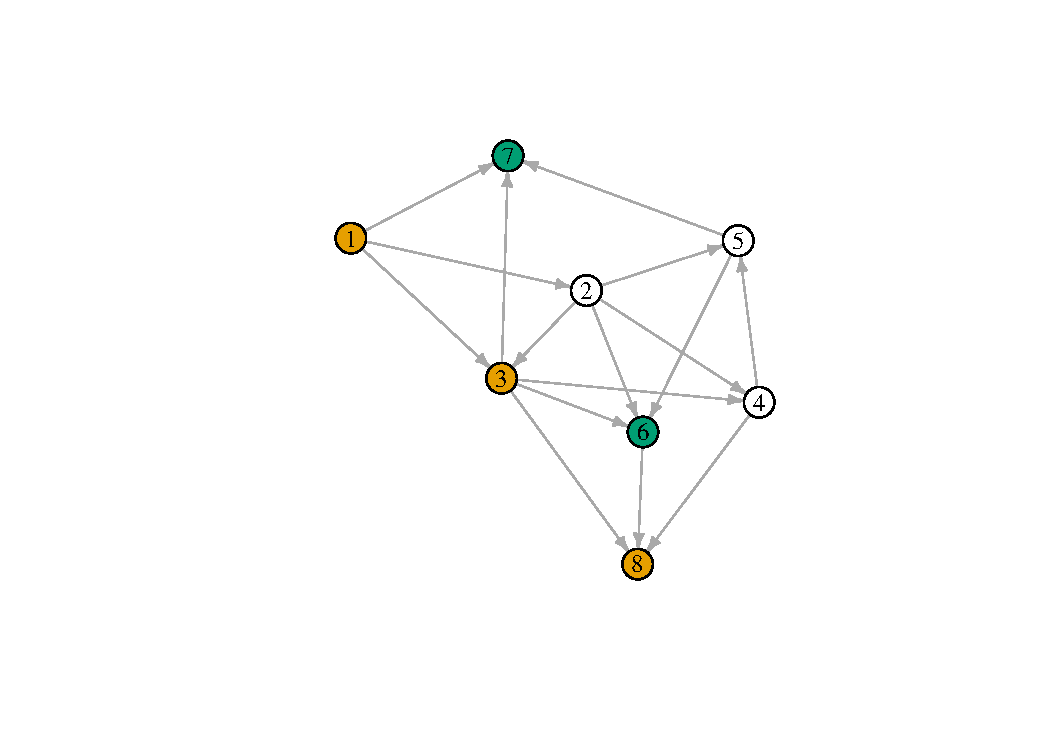
\includegraphics{report_pdf_files/figure-latex/unnamed-chunk-1-1.pdf}

\subsection{Idea of the algorithm}\label{idea-of-the-algorithm}

We formulate the problem in terms of paths (routes) between o-d pairs.
The simplicial decomposition approach can be viewed as a column
generation approach. Consider a subset of k paths , we solve a master
problem (MP) and evaluate this solution to other problem. If optimal
path flows are optimal in MP are also optimal in other problem. The idea
is to evaluate the arc flows and the gradient of the objective function.
By the Caratheodory theorem, any feasible point of bounded polytype can
be expressed as a convex combination of its extreme points, and it's
obtained by the MP.

The quadratic function to minimize is:
\(\displaystyle \sum c_{ij}\;x + \displaystyle \sum \frac{1}{2} d_{ij} \;x^2\)
subject to supply the o-d pairs flow in the network.

\subsection{Introduction}\label{introduction-1}

The class of simplicial decomposition (SD) schemes have shown to provide
efficient tools for nonlinear network flows. Shortest subproblems are
solved in order to generate extreme points of the polyhedron of feasible
flows, and, alternately, master problems are solved over the convex hull
of the generated extreme points. We review the development of simplicial
decomposition and the closely related column generation methods.

Simplicial decomposition (SD) algorithms based on Carathéodory's theorem
(modification of Frank-Wolfe). A direct consequence of this theorem is
that any point in a bounded polyhedral set X can be described by a
convex combination of its extreme points. In SD algorithms, extreme
points are generated algorithmically by the solution of the linear
Frank-Wolfe subproblem. Alternately, a so called master problem, defined
by a restricted set of extreme points, is solved in order to generate a
new iteration point.

Steps of the algorithm:

\begin{enumerate}
\def\labelenumi{\arabic{enumi})}
\tightlist
\item
  Solve subproblem (gradient of the objective function):
  \(c_{ij} + d_{ij}\;x\).
\end{enumerate}

First we solve the subproblem with an initial value of \(t0 = 1\) to
generate a bad initial solution of the Sub-Problem. After that we
increase the sets \textbf{Ws} and then solve the \textbf{Master Problem}
(MP). With the values of the \textbf{MP} whe are going to fix a new
value to \(t0\) based on the gradient of the \textbf{quadratic function}
evaluated in \textbf{vv} obtained in the resolution of \textbf{MP} where
\textbf{vvv} is the sets \textbf{Wx} multiplied by their associated
\(\alpha_{i = 1..n}\).

\begin{enumerate}
\def\labelenumi{\arabic{enumi})}
\setcounter{enumi}{1}
\tightlist
\item
  Update working sets: Add new vertex and remove with information of
  \(\alpha\) (MP variable) the smaller baricentric coordinate (small
  value of \(\alpha\)). When we say small is in terms of zero or
  closeness to zero.
\end{enumerate}

When we arrive at a point where the dimensions of \textbf{Ws} is equal
to \textbf{rho} we have to modify the columns of \textbf{Ws} based on
the the associated values of \(\alpha\). To do that we will choose the
smallest value of vector of \(\alpha\) (associated to the baricentric
coordinates of vertexs) and change this column with the value obtained
in the new resolution of \textbf{SP}.

\begin{enumerate}
\def\labelenumi{\arabic{enumi})}
\setcounter{enumi}{2}
\tightlist
\item
  Update best lower bound (BLB) and calculate gap. When the \textbf{GAP}
  will be close to zero or the number of iterations arrive to 500 the
  algorithm will stop.
\end{enumerate}

In step 3, we will update the \textbf{BLB} as:
\(max(BLB,f(x^v)+\nabla_xf(x^v)^T(\hat{x}^v-x^v))\) and gap as:
\(\frac{f(x^v-BLB)}{BLB}\). With this criterion we will ensure that our
\textbf{BLB} and the value of the \textbf{f.obj} will converge and the
gap will tend to zero.

We stop iterating if \(gap < 0.005\) or iteration number is equal to
500.

\begin{enumerate}
\def\labelenumi{\arabic{enumi})}
\setcounter{enumi}{3}
\tightlist
\item
  Solve MP: Minimize quadratic function subject to actual working set,
  or in other words, solve problem with a convex combination of extreme
  points obtained in previous steps. \emph{Go to step 1}.
\end{enumerate}

At this point, we will use the set of combinations, called \textbf{W}
(solutions obtained solving at each step the SP) to solve the MP and
obtain the optimal solution of the algorithm or new points (combinations
of origen destination flows) to use in the SP as a combination of origen
destination flows multiplied by \(\alpha_{i = 1..n}\).

We start algorithm with \textbf{BLB} = \(-\infty\). The goal is to
observe how the \textbf{MP} and \textbf{BLB} will become closer at every
iteration.

\subsubsection{Procedure information}\label{procedure-information}

\begin{itemize}
\tightlist
\item
  nº iter
\item
  Funcio objectiu Q
\item
  relgap value
\item
  step length ?
\item
  nº vertexs
\item
  Size of working sets Wx, Ws
\end{itemize}

\subsubsection{Graphical representation of
procedure}\label{graphical-representation-of-procedure}

\begin{itemize}
\tightlist
\item
  iter vs lower bound
\item
  iter vs log(relgap)
\end{itemize}

\subsection{Direct solution}\label{direct-solution}

Let's start solving the problem directly. The objective function found
is 17.350. With this value we will now the aproximate value of the
solution of \textbf{RSD} algorithm (i say aprox. because our GAP is not
zero). We display the values of the amount that is moved between the
diferent \textbf{O-D} pairs and the value of the objective function
returned by the algorithm. Is important to remember that in easy
problems the algorithm solved by this method (let's call them the
simplest method) could be obtained, while in long problems will be
imposible to know this value.

\subsection{Printout of the
iterations}\label{printout-of-the-iterations}


\end{document}
